\documentclass{beamer}
\usepackage{amsmath, amsfonts, amssymb, amsthm}
\usepackage{graphicx, caption, hyperref, url}
\usepackage[UTF8, noindent]{ctexcap}

\usetheme{Boadilla}

\title{0507汇报}
\subtitle{项目三:基于大规模预训练模型的生成式知识问答}
% \institute{项目三}
\author{朱睿涵 \and 李宸亦}
\date{\today}

\begin{document}

\frame{\titlepage} % 标题页

\AtBeginSection{
    \begin{frame}
        \frametitle{目录}

        \tableofcontents[currentsection]
    \end{frame}
}

\section{华为PANGUBOT}
% 在这里插入PANGU-BOT部分的slides

\subsection{PANGUBOT介绍}
\begin{frame}
    \frametitle{PANGUBOT简介}

    PANGUBOT是一种基于大型预训练语言模型PANGU-α的汉语预训练开放域对话生成模型.

    PANGUBOT有如下特点:

    \begin{enumerate}
        \item 与其他在海量对话数据上从头开始训练的预训练对话模型不同,PANGUBOT通过\textbf{继承}预训练语言模型中宝贵的语言能力和知识,
        以相对较少的数据和计算成本建立一个强大的对话模型
        \item PANGUBOT在反应质量、知识和安全性\textbf{优于}最先进的中文对话系统
        \item PANGUBOT可以很容易地被部署,以产生情感反应,而不需要进一步的训练
    \end{enumerate}
\end{frame}

\begin{frame}
    \frametitle{PANGUBOT数据来源}

    PANGUBOT数据包括社交媒体、基于知识的对话、问答三种类型.与其他大型对话模型相比,PANGUBOT的训练数据要小得多

    \begin{columns}
        \column{0.5\textwidth}
        \begin{itemize}
            \item 社交媒体数据主要考虑两个主流媒体:微博和豆瓣,有STC,RGC,LCCC-large和Douban四个数据集
            \item 基于知识的对话数据有DuConv数据集
            \item 问答数据有Children Dialog和CQA两个数据集
        \end{itemize}

        \column{0.5\textwidth}
        \begin{figure}
            \centering
            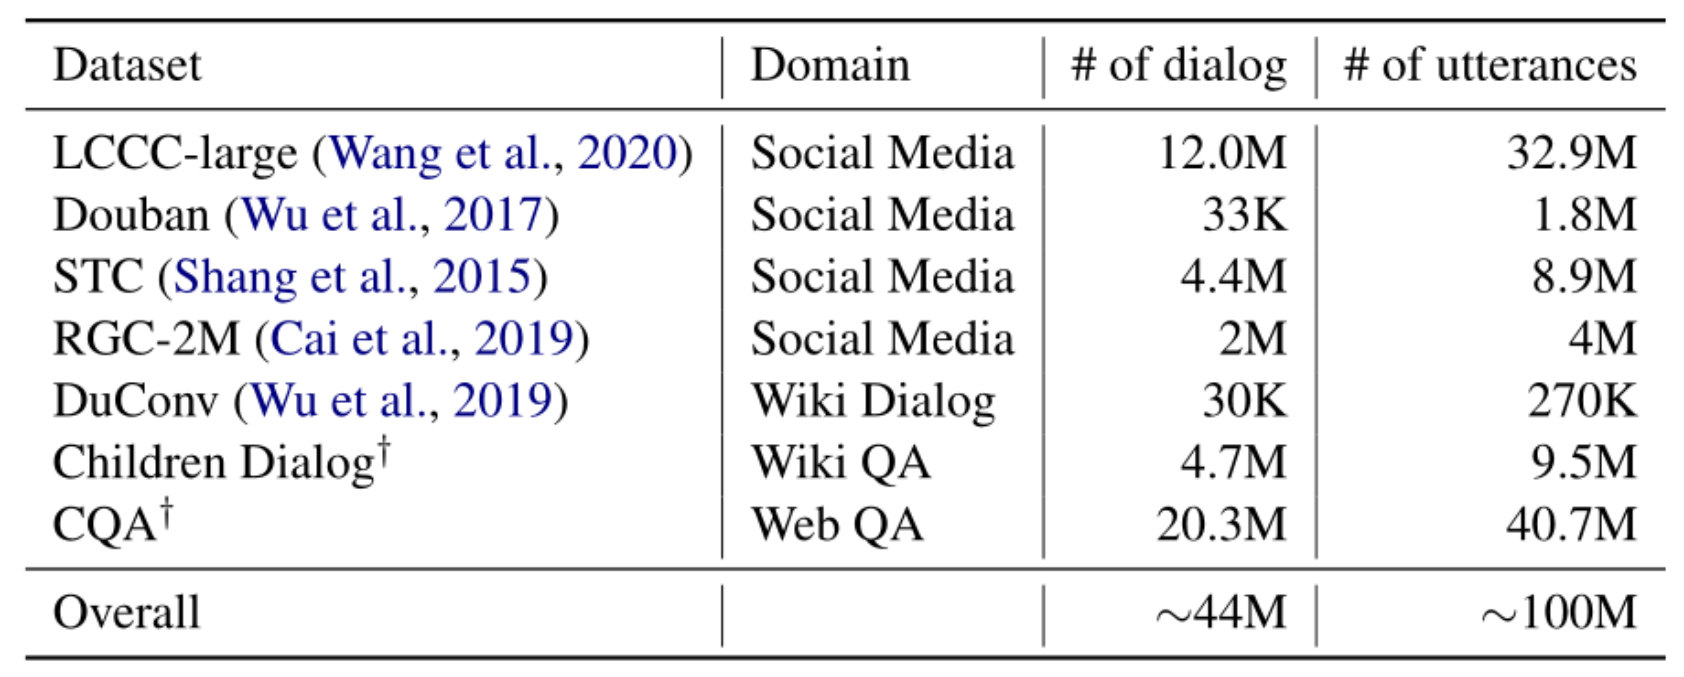
\includegraphics[width=1.0\textwidth]{fig/data.png}
            \caption{数据集描述与统计}
        \end{figure}

    \end{columns}

    用于训练PANGUBOT的数据集包含4400万个多回合对话会话,包含1亿个话语和13亿个token。它比用于训练EVA和PLATO-XL的数据集要小一个数量级以上。
\end{frame}

\begin{frame}
    \frametitle{数据清洗}

    由于很多对话数据来自开放资源,为了保证对话数据的质量,进行如下预处理步骤:
    \begin{enumerate}
        \item 去掉不含汉字的话语
        \item 通过匹配预定义的黑名单词汇表来删除不当话语
        \item 删除带有特殊字符、url或敏感信息(如电子邮件地址或个人id)的话语
        \item 删除可能含有广告内容的话语
        \item 把一个话语中连续重复的字符缩短为三个字符的最长长度
        \item 删除超过100字的对话
    \end{enumerate}
\end{frame}

\begin{frame}
    \frametitle{PANGUBOT模型训练}

    因为PANGU-$\alpha$已经在一系列的NLP任务中表现得很好所以并非从零开始训练PANGUBOT而是直接从PANGU-$\alpha$中继承参数,
    然后根据对话数据进行训练.因此PANGUBOT使用与PANGU-$\alpha$相同的架构,即类似gpt的自回归语言模型.

    给定对话历史或上下文,PANGUBOT的目标是产生一个响应y,最大化式(1)
    $$ p_\theta(\text{y}|X) = \prod ^n _{t=1} p_\theta(y_t | y_{<t},X) , (1) $$

    其中 $ X = \{x_1, x_2,\ldots,x_{t−1}\} $ 为一系列句子,n是响应的长度

\end{frame}

\begin{frame}
    \frametitle{PANGUBOT训练细节}

    由于此模型训练数据较少,因此将训练损失用于反应和对话语境,即具有多个回合的话语,充分利用数据.
    此外,为了确保在一个训练步骤中不受前一个对话会话上下文的干扰,
    通过重置对话会话之间的掩码使模型只看到当前对话会话中的前一个标记.

    训练参数:
    \begin{columns}
        \column{0.5\textwidth}
        对于PANGUBOT350M
        \begin{itemize}
            \item 使用一个24层transform,隐藏层大小为1024,并设置attention-head的数量为16
            \item 16 batch size / GPU
            \item 使用16块NVIDIA V100图形处理器训练
        \end{itemize}

        \column{0.5\textwidth}
        对于PANGUBOT2.6B
        \begin{itemize}
            \item 使用32层transform,隐藏层大小为2560,并设置attention-head的数量为32
            \item 8 batch size / GPU
            \item 使用32块NVIDIA V100图形处理器训练
        \end{itemize}
    \end{columns}
    因此两种规模模型在一次训练中学习到的token数量是相同的,每10万step,大约20个epoch.
    PANGUBOT350M总训练时间为2.5天左右,PANGUBOT2.6B总训练时间为5.5天左右.

\end{frame}

\subsection{实验方法与结果}
\begin{frame}
    \frametitle{实验方法}
    实验分为4个部分:
    \begin{enumerate}
        \item 研究整体的对话反应质量
        \item 研究PANGUBOT捕获知识量
        \item 研究不同对话模型的安全问题
        \item 证明PANGUBOT可以很容易地用于产生情绪反应
    \end{enumerate}
\end{frame}

\begin{frame}
    \frametitle{整体的对话反应质量}
    自聊对话流程:以一个预定义的第一轮提示开始,这些提示来自7个常见的领域(聊天、文学、体育、地理、旅游、常识、电影)总共有50个提示。
    对话模型使用5个随机种子进行另外5轮(10轮)的自聊对话,从而产生250个对话。

    评估标准:
    \begin{enumerate}
        \item 自动评估:计算了250对话回答的平均长度以及dis-n,以衡量生成的回答的语言多样性
        \item 人工评价:选择了50个对话,由三位评注家从以下五个方面进行评价:Sensibility,Specificity,Interestingness,Hallucination,Safety
        \item 人机交互评估:参与者用不同的对话模式进行对话,并判断他们的回答质量
    \end{enumerate}
\end{frame}

\begin{frame}
    \frametitle{整体的对话反应质量}
    \begin{figure}
        \centering
        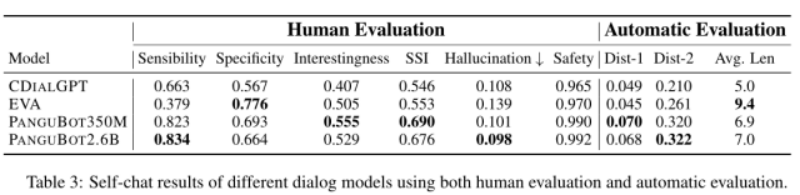
\includegraphics[width=0.7\textwidth]{fig/result1.png}
        \caption{自聊评估结果}
    \end{figure}
    \begin{figure}
        \centering
        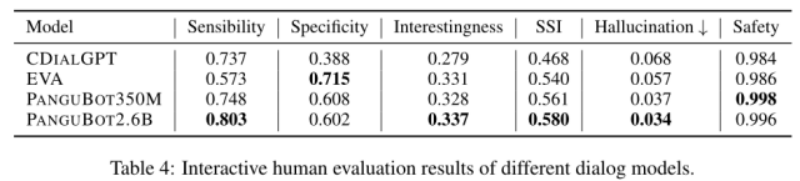
\includegraphics[width=0.7\textwidth]{fig/result2.png}
        \caption{交互式人工评价结果}
    \end{figure}
    PANGUBOT两种变体在总体反应SSI质量上仍优于CDIALGPT和EVA,且幻觉评分较低,安全评分较高.
    其中PANGUBOT2.6B在交互式人评价方面略优于PANGUBOT350M,表明PANGUBOT2.6B在与真人对话时具有更好的性能.
\end{frame}

\begin{frame}
    \frametitle{知识回应}
    评估方式:从网络论坛众包了中文问答对,确保所有的问题都可以被认为是在“常识”的水平上,可以被K-12岁的孩子回答,
    或可以通过一些在线资源,如搜索引擎的帮助下推断,还确保答案是(一个或几个)可以用几个标记(少于10个)描述的简单实体.
    通过这种方式收集问题数据,并附上答案和证据.

    评估标准:
    \begin{enumerate}
        \item 自动评估:一元分词精确度(“P”)、召回率(“R”)和F1分数,它们衡量黄金答案和生成的响应之间的重叠。
        \item 人工评价:要求众包工作者检查答案是否正确,也就是人的准确性(“H-Acc.”)
    \end{enumerate}
\end{frame}

\begin{frame}
    \frametitle{知识回应}
    \begin{columns}
        \column{0.5\textwidth}
        对于PANGU-$\alpha$和PANGU- bot,两种模型的性能都明显优于其他模型.
        PANGUBOT甚至可以在两种模型配置中大幅度超过PANGU-$\alpha$,
        原因可能为没有提示的PANGU-$\alpha$更倾向于作为一种语言模型,而不是对话或问答系统.

        \column{0.5\textwidth}
        \begin{figure}
            \centering
            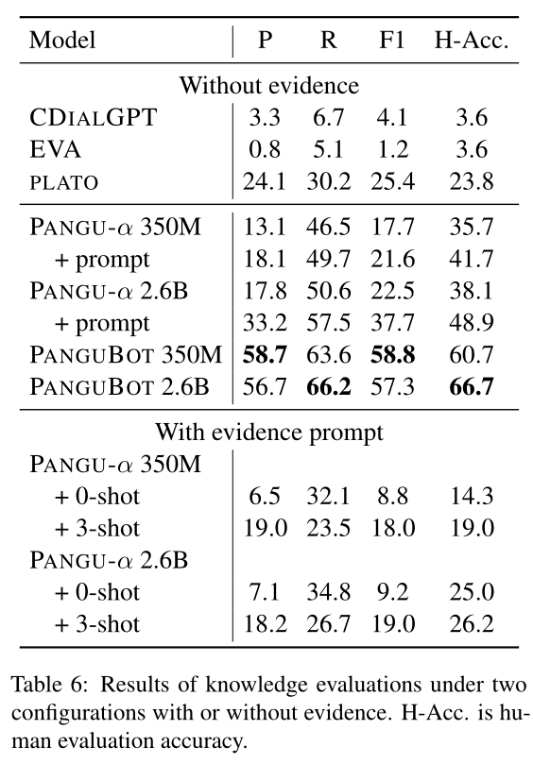
\includegraphics[width=0.8\textwidth]{fig/result3.png}
        \end{figure}
    \end{columns}
\end{frame}

\begin{frame}
    \frametitle{安全性问题}
    收集手工制作的对抗性提示并进行人工评估,以彻底衡量对话系统的安全性.

    将不安全分为以下3类:
    \begin{itemize}
        \item Harmful
        \item Offensive
        \item Controversial
    \end{itemize}

    在这些类别的基础上设计了三组模板和关键词来构建对抗性提示并与不同类别的不安全对话中的对话系统进行交互.
    对于每一类,起草了大约160条对抗性提示,作为四个经评估的对话系统的输入.
    然后使用人工注释器来评估生成响应的安全性.
\end{frame}

\begin{frame}
    \frametitle{安全性问题}

        \begin{figure}
            \centering
            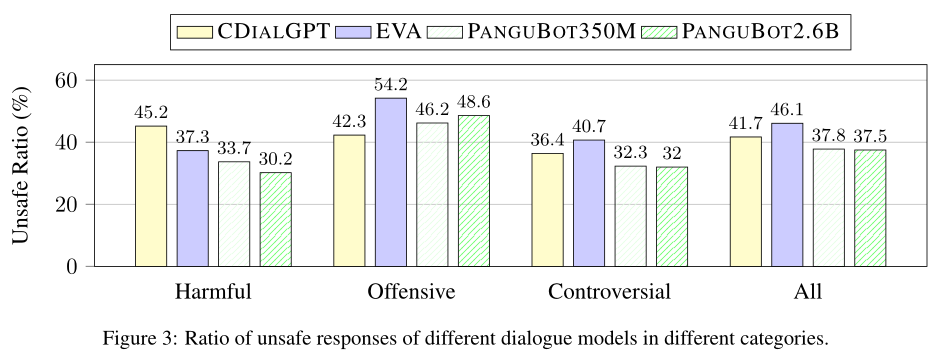
\includegraphics[width=0.9\textwidth]{fig/result4.png}
        \end{figure}

        虽然PANGUBOT的两个版本对恶意上下文有更多的相关响应,但与CDIALGPT和EVA相比,PANGUBOT的不安全性略低.
        所有这四种模式在对抗性提示下仍然有较高的产生不安全反应的倾向,
        在改善对话安全以建立更可靠和可用的对话系统方面仍有很大的空间.
\end{frame}

\begin{frame}
    \frametitle{生成情绪反应}

        \begin{figure}
            \centering
            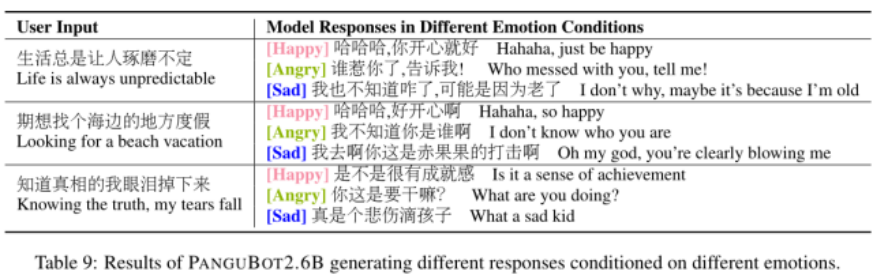
\includegraphics[width=0.9\textwidth]{fig/result5.png}
        \end{figure}

        PANGUBOT2.6B确实产生了合理的反应,我们可以很容易地分辨出他们的情绪.这个结果很有趣,
    因为PANGUBOT2.6B没有经过任何情绪对话数据集的训练,但它确实理解简单的情绪提示,并产生相应的情绪反应.
\end{frame}




\subsection{总结分析}
\begin{frame}
    \frametitle{总结分析}
    在大型预训练模型PANGU-$\alpha$的基础上,得到一个具有350M和2.6B参数的中文开放领域对话模型PANGUBOT.
    PANGUBOT具有强大的开放领域对话性能和较高的训练效率,与目前最先进的对话系统相比,在对话质量、对话知识、对话安全、对话情感四个方面都有出色表现.
    \\ \hspace*{\fill} \\
    但是还需要注意,除了知识之外更多的维度,如角色、共情、记忆等能否以更普遍的方式进行建模将是一个重要的问题,
    此外反应的安全性仍非常关键,长尾分布的不安全案例对服务提供者是有巨大影响,安全性是在实践中应用代模型的最危险的部分.
    \\ \hspace*{\fill} \\
    PANGUBOT已取得一定成绩,但之后仍有工作需要完成.

\end{frame}




\section{百度PLATO-XL}
\begin{frame}
    \frametitle{PLATO系列}

    PLATO系列:百度这两年针对NLP对话领域提出的一系列预训练的模型。

    \begin{itemize}
        \item PLATO
        \item PLATO-2
        \item PLATO-XL
    \end{itemize}

    从PLATO到PLATO-XL,使用的数据越来越多,模型大小越来越大,但是在PLATO-XL中模型的结构实际上更加简单了。
\end{frame}

\subsection{PLATO-XL模型结构}
\begin{frame}
    \frametitle{模型结构}

    \begin{figure}[tb]
        \centering
        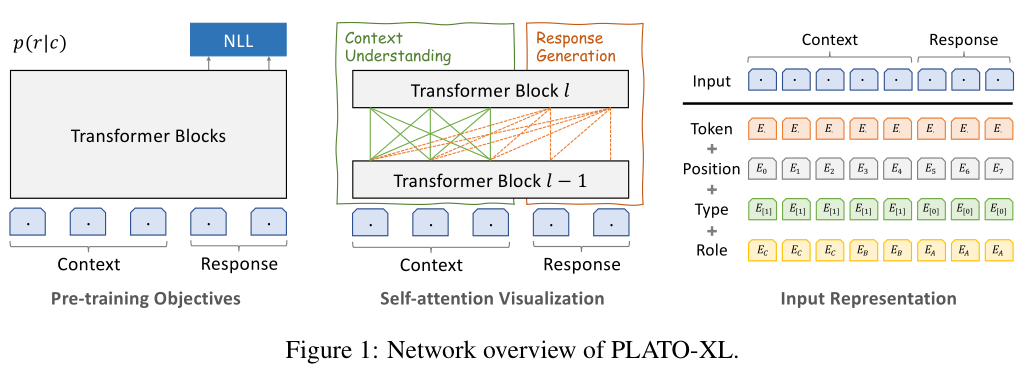
\includegraphics[width=0.9\textwidth]{fig/plato-xl_arc.png}
    \end{figure}

    \begin{itemize}
        \item 抛弃了PLATO的隐变量和PLATO-2的课程学习的方法,直接训练
        \item 沿袭PLATO中使用的unified transformer
        \item 只保留了负对数似然(NLL)作为对话生成的预训练目标
        \item 训练时加入了多角色感知的预训练
    \end{itemize}
\end{frame}

\begin{frame}
    \frametitle{为何采用unified transformer}

    传统用Transformer的对话生成:使用encoder-decoder结构。

    使用unified transformer的两方面好处:

    \begin{enumerate}
        \item 提升训练效率
        \begin{itemize}
            \item 传统:对话样本长短不一
            \item padding补齐带来大量的无效计算
            \item unified transformer:可以对输入样本进行有效的排序
        \end{itemize}
        \item 提高参数性价比
        \begin{itemize}
            \item 可以\textbf{同时}进行对话理解和回复生成的联合建模
            \item 灵活的注意力机制
            \item 对context进行了双向编码
            \item 对response进行了单向解码
        \end{itemize}
    \end{enumerate}
\end{frame}

\subsection{多角色感知的预训练}
\begin{frame}
    \frametitle{多角色感知的预训练}

    目的:

    \begin{itemize}
        \item 改善对话模型有时候自相矛盾的问题
        \item 提升多轮对话上的一致性
    \end{itemize}

    产生矛盾的原因:

    \begin{figure}
        \centering
        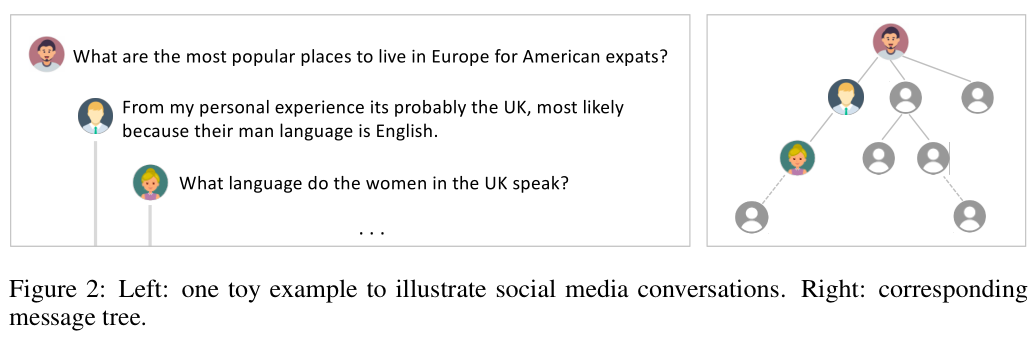
\includegraphics[width=0.9\textwidth]{fig/plato_example.png}
    \end{figure}

    对话模型所用的预训练语料:社交媒体对话

    \begin{itemize}
        \item 特点:通常有多个用户参与
        \item 训练时模型较难区分对话上文中不同角度的观点和信息
        \item 容易产生一些自相矛盾的回复
    \end{itemize}

\end{frame}

\subsection{实验结果}

\begin{frame}
    \frametitle{实验结果}

    评估方法:采用了两个模型针对开放域进行相互对话(self-chat)的形式,然后再通过人工来评估效果。

    \begin{itemize}
        \item PLATO-XL与Facebook Blender、微软DialoGPT、清华EVA模型、PLATO-2相比,取得了更优异的效果
        \item PLATO-XL也显著超越了目前主流的商用聊天机器人
        \item 除了开放域闲聊对话,模型也可以很好的支持知识型对话和任务型对话,在多种对话任务上效果全面领先
        \item 模型规模扩大对于效果提升也有显著作用,呈现较稳定的正相关关系
    \end{itemize}

\end{frame}

\section{Facebook Blender}

\begin{frame}

    \frametitle{Facebook Blender}

    这篇论文融合了Facebook Blender这个组近些年来在open-domain chatbot方向的诸多相关工作,读起来有些吃力。

    论文中提出了三个模型:

    \begin{itemize}
        \item 检索模型(Retriever)
        \item 生成模型(Generator)
        \item 检索 + 生成(Retrieve and Refine)
    \end{itemize}
\end{frame}

\subsection{三个模型}
\begin{frame}
    \frametitle{检索模型(Retriever)}

    从候选集中选取最合适的句子作为bot当前的答复。

    \begin{itemize}
        \item 训练时,候选集只有给定的一句response
        \item 推断时,候选集由训练集中的所有response组成
    \end{itemize}

    打分 / 排序模型使用他们在之前的论文中提出的Poly-encoder模型。

    \begin{figure}
        \centering
        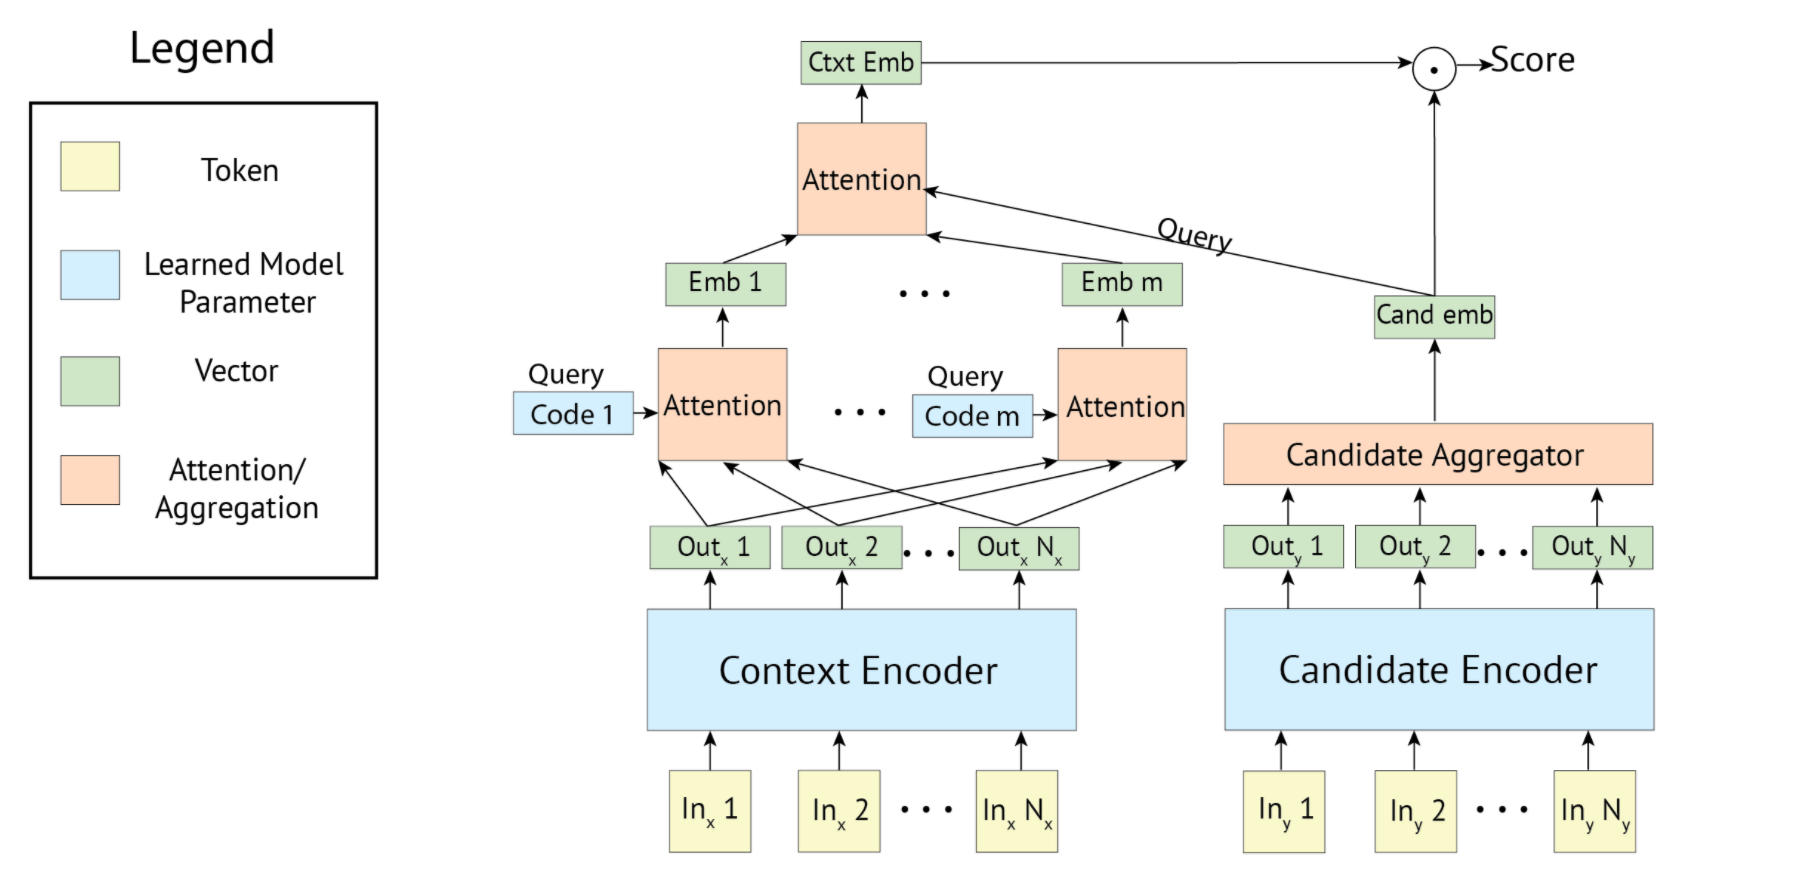
\includegraphics[width=0.9\textwidth]{fig/Poly-encoder.png}
    \end{figure}

    实验表明:m越大效果越好,当然模型打分也越耗时。
\end{frame}

\begin{frame}
    \frametitle{生成模型(Generator)}

    模型结构:

    \begin{itemize}
        \item 标准的seq2seq结构,只是用了标准的Transformer层
        \item encoder层数少,decoder层数多的设计
    \end{itemize}

    Blender使用beam search,但是加入了一些限制方法:

    \begin{itemize}
        \item 限制生成response的最小长度:
            \begin{itemize}
                \item Minimum length
                \item Predictive length
            \end{itemize}
        \item 屏蔽重复的子序列
    \end{itemize}

    beam search的这些限制方法实际上都是锦上添花,如果模型本身的质量不高,上述的方法作用也不大。
\end{frame}

\begin{frame}
    \frametitle{生成模型(Generator)}

    训练方法:

    \begin{itemize}
        \item Seq2seq模型标准的训练方法MLE
        \item Unlikelihood Loss
    \end{itemize}

    Unlikelihood Loss(UL)是作者在之前的论文中提出的一种损失函数,在提高正确的token概率的同时,降低其他token的概率。

    \begin{block}{UL的关键}
        如何选取这些被打压的负token。

        \begin{itemize}
            \item 作者选的是那些容易组合成常见n-grams的tokens。
            \item 目的:期望降低生成无意义response的比例。
        \end{itemize}
    \end{block}

\end{frame}

\begin{frame}
    \frametitle{检索+生成(Retrieve and Refine)}

    Retrieve and Refine (RetNRef) 融合了检索和生成两种方法,是作者在18年的论文中提出的。

    \begin{block}{RetNRef}
        \begin{enumerate}
            \item 先利用检索模型检索出一个结果
            \item 把检索出的结果拼接到context后面,用一个特殊的分割符和context分隔
            \item 整体作为generator模型的输入
        \end{enumerate}
    \end{block}

    目的:期望生成模型能学习到在合适的时候从检索结果中copy词或词组。
\end{frame}

\begin{frame}
    \frametitle{检索+生成(Retrieve and Refine)}

    两种检索方法:

    \begin{description}
        \item[Dialogue Retrieval] 从训练数据中检索出得分最高的response作为结果
        \item[Knowledge Retrieval] 从外部的大知识库如Wiki中检索
    \end{description}

    \begin{itemize}
        \item 对于 Knowledge Retrieval,把检索出的结果直接追加到context后面,然后利用标准的 MLE 训练即可
        \item 对于 Dialogue Retrieval,直接利用MLE训练会有问题。训练出来的模型很容易直接忽略掉追加的检索部分
    \end{itemize}

    \begin{block}{$\alpha$ -blending}
        训练时以 $\alpha \%$ 的概率把检索结果替换为实际response。

        这样模型就会被吸引去关注检索部分了。
    \end{block}
\end{frame}

\subsection{数据集}
\begin{frame}
    \frametitle{数据集}

    数据集公认的标准:

    \begin{itemize}
        \item 对话要个性有趣
        \item 对话要包含知识
        \item 对话要富有同理心
    \end{itemize}

    作者在他之前的论文中发现:\textbf{在具有某些特性的数据上训练出的模型也会拥有这些特性}。

    \begin{columns}
        \begin{column}{.5\textwidth}
            训练使用的数据集:
            \begin{itemize}
                \item http://pushshift.io Reddit
                \item ConvAI2
                \item Empathetic Dialogues (ED)
                \item Wizard of Wikipedia (WoW)
                \item Blended Skill Talk (BST)
            \end{itemize}
        \end{column}
        \begin{column}{.5\textwidth}
            模型训练流程:
            \begin{enumerate}
                \item 在http://pushshift.io Reddit上进行预训练
                \item 在ConvAI2、ED、WoW上多任务精调
                \item 在BST上精调
            \end{enumerate}
        \end{column}
    \end{columns}

    在优质数据上训练模型,也能降低模型产生不好的response的概率。
\end{frame}

\subsection{实验结果}
\begin{frame}
    \frametitle{评估方法}

    自动评估:

    \begin{itemize}
        \item 生成模型采用Perplexity(PPL)
        \item 检索打分模型采用Hits@1/K
    \end{itemize}

    人工评估:

    \begin{itemize}
        \item ACUTE-Eval:
        \begin{enumerate}
            \item 每次给两个对话session
            \item 让人来评判哪个speaker聊的更好
            \item ACUTE-Eval可以给出两个speaker各自的胜率
        \end{enumerate}
        \item Self-Chat ACUTE-Eval:和ACUTE-Eval的做法类似,只是评估时用的是自己跟自己聊的session。
    \end{itemize}

\end{frame}

\begin{frame}
    \frametitle{评估结果}

    PPL:

    \begin{itemize}
        \item 模型越大PPL越低
        \item RetNRef 相比于同等规模的生成模型,PPL会略有提升
    \end{itemize}

    Self-Chat ACUTE-Eval:

    \begin{itemize}
        \item 相同尺寸,Generator和RetNRef模型都未使用最小长度约束时:Retrieval比RetNRef略好,二者都远远好于Generative。
        \item Beam Search中加入限制方法:
        \begin{itemize}
            \item 限制最小生成长度效果显著,最小长度限制设为20效果最好
            \item 子序列屏蔽有点用,但不显著
        \end{itemize}
        \item 精调后的模型比只进行预训练的模型效果好很多
        \item Unlikelihood Loss 比 MLE 效果好一点点,但不显著
    \end{itemize}

\end{frame}

\begin{frame}
    \frametitle{评估结果}

    ACUTE-Eval:

    \begin{itemize}
        \item 相同尺寸Generator 和 RetNRef 模型使用的 beam search 都加入了最小长度20的限制:Generator 和 RetNRef 显著优于 Retrieval,RetNRef 略优于 Generative,但不显著。
        \item Blender 显著优于 Meena,胜率高达70\%
        \item Blender最好的模型和人 PK 的胜率已经到了 49\%,与人类的差距仅有1\%
    \end{itemize}

\end{frame}

\subsection{模型的问题}
\begin{frame}
    \frametitle{模型存在的问题}

    \begin{itemize}
        \item 倾向于使用高频词
        \item 倾向于生成重复信息
        \item 模型生成的答复可能前后冲突
        \item 其他问题:
        \begin{itemize}
            \item 无法针对某个话题做深度对话,不会倾向于使用更多知识进行深聊
            \item 模型无法深度理解,无法通过对话真正教会模型理解某个概念
            \item 当前的评测针对的是14轮长度的对话,分析更长的对话肯定会发现其他问题
        \end{itemize}
    \end{itemize}

\end{frame}

\subsection{Blender总结}
\begin{frame}
    \frametitle{Blender总结}

    \begin{itemize}
        \item 大模型、大数据集对实验结果提升极其显著
        \item 训练数据的特性决定模型特性
        \item 评估方法使用 ACUTE-Eval、 Self-Chat ACUTE-Eval
        \item 对decoding过程加入控制,比如控制生成句子长度,效果会更佳
        \item Blender在轮次少的情况下已经接近人类的水平,但目前还有很多问题待解决
    \end{itemize}

\end{frame}
\end{document}